\chapter{制約充足問題} \label{chap:CSP}
制約充足問題(Constraint Satisfaction Problem, CSP)は, 計算量理論において重要な問題の一つであり, PCP定理の証明においても中心的な役割を果たす.

\section{制約充足問題の定義}
制約充足問題とは端的に言えば連立方程式の解の存在性判定を問う判定問題である.

\begin{definition}{制約充足問題}{CSP}
\emph{制約充足問題(CSP)}とは次の要素からなる組$\varphi = (X,\Sigma,\calI,\calC)$を入力とする判定問題である:
\begin{itemize}
  \item \emph{アルファベット}と呼ばれる有限集合$\Sigma$.
  \item 変数集合$X=\{x_1,\dots,x_n\}$.
  \item 部分集合族$\calI=\{I_1,\dots,I_m\}$. ただし各$I_i$は$I_i\subseteq[n]$である.
  \item 関数族$\calC=\{c_1,\dots,c_m\}$. ただし各$c_i$は$c_i: \Sigma^{I_i}\to\{0,1\}$である.
\end{itemize}
入力$(X,\Sigma,\calI,\calC)$は,
ある変数への割り当て$(a_1,\dots,a_n)\in\Sigma^n$が存在して, 任意の$i\in[m]$について$c_i(a_{I_i})=1$であるとき, かつその時に限りYesインスタンスである.
ここで, $a_{I_i}=(a_{i_1},\dots,a_{i_{\abs{I_i}}})$は$a_i$の部分列である.
特に, 全ての$i\in[m]$について$\abs{I_i}\le q$であるとき, このCSPは\emph{$q$-CSP}という.

また, 固定した割り当て$\veca = (a_1,\dots,a_n)$に対する$\varphi$の\emph{充足度}を
\begin{align*}
  \val(\veca) = \Pr_{i\sim[m]}[c_i(\veca_{I_i})=1]
\end{align*}
とし, 全ての割り当てに関して充足度の最大値
\begin{align*}
  \val(\varphi) = \max_{\veca\in\Sigma^n} \val(\veca)
\end{align*}
を$\varphi$の充足度という.
\end{definition}

\begin{example}{グラフ彩色問題}{graph-coloring-problem-CSP}
  グラフ彩色問題(\cref{ex:graph-coloring-problem})は$2$-CSPである.
  実際, グラフ$G=(V,E)$に対して
  \begin{itemize}
    \item 変数集合を$X=V$とする.
    \item アルファベットを$\Sigma=[k]$とする.
    \item 制約集合を$\calI=\{E\}$とする.
    \item 関数族を$\calC=\{c_e\}_{e\in E}$とし, 各$e=\{u,v\}\in E$に対して
    \begin{align*}
      c_e(a_u,a_v) = \begin{cases}
        1 & \text{if } a_u\neq a_v, \\
        0 & \text{if } a_u=a_v
      \end{cases}
    \end{align*}
    と定義する.
  \end{itemize}
  このとき, グラフ$G$が$k$-彩色可能であることと, このCSPがYesインスタンスであることは同値である.
\end{example}


\subsection{PCPとの関係}
ランダムシード長$r=r(n)$かつクエリ数$q=O(1)$のPCP検証者は$\Sigma=\{0,1\}$の場合の$q$-CSPによって表現でき, 逆に$q$-CSPはPCP検証者として表現できる.
実際, $q$クエリのPCP検証者$V^\pi(x)$を考えよう.
証明の長さを$\abs{\pi}=\ell$とする.
入力$x$とランダムシード$s$を固定したときの$V^\pi(x;s)$が
証明中の読み込む文字のインデックスの集合を$I_s\subseteq[\ell]$とする (ここで$\abs{I_s}\le q$).
このとき, $V^\pi(x;s)$は$\binset^{I_s}$を$\binset$に写す関数を定める.
この関数を制約$c_s$とみなすことで, 検証者$V^\pi(x)$は$q$-CSPのインスタンスとして表現できる.
このとき, $q$-CSPのインスタンスの変数集合は証明$\pi$に対応する.
もし$x\in L$であるならば, 確率$1$で$V^\pi(x)=1$となるような$\pi$が存在する.
つまり, 全てのランダムシード$s$に対して$V^\pi(x;s)=1$となるような$\pi$が存在するため,
先ほど構成した$q$-CSPのインスタンスはYesインスタンスである.
逆に$x\not\in L$であるならば, 全ての$\pi$に対して確率$1/3$以上で$V^\pi(x)=0$となる.
これは, $q$-CSPインスタンスに対して, 全ての割り当てを考えても, 全体の制約のうち少なくとも$1/3$の割合は充足されないことを意味する.


\begin{table}[htbp]
  \centering
  \begin{tabular}{|c|c|}
    \hline
    PCP検証者 & $q$-CSP \\
    \hline
    PCP $\pi$ & 割り当て \\
    \hline
    ランダムネスを固定した時の判定 & CSPの制約 \\
    \hline
    PCP$\pi$を受理する確率 & 割り当ての充足度 $\val(\pi)$ \\
    \hline
  \end{tabular}
  \caption{PCPとCSPの対応関係}
  \label{table:pcp-csp-correspondence}
\end{table}

この対応関係に基づいて, PCP定理をCSPを用いた言葉で表すことができる.

\begin{theorem}{PCP定理のCSP版}{PCP-CSP-theorem}
  ある関数$m=n^{O(1)}$, $q=O(1)$, $\ell=n^{O(1)}$, 定数$c\in\Nat$, $\epsilon>0$, および
  次の性質を満たす多項式時間決定的アルゴリズム$A$が存在する:
  3彩色問題のインスタンス$G=(V,E)$を入力として受け取り, $G$の頂点数を$n$としたとき, $A$は高々$\ell(n)$個の変数と$m(n)$個の制約および要素数$c$のアルファベットからなる$q$-CSPのインスタンス$\varphi$を出力する.
  さらにこのインスタンス$\varphi$は
  \begin{itemize}
  \item 入力$G$が$\ThreeCOL$のYesインスタンスであるとき, $\val(\varphi) = 1  $となる (すなわち$\varphi$はYesインスタンス).
  \item 入力$G$が$\ThreeCOL$のNoインスタンスであるとき, $\val(\varphi) < 1-\epsilon$となる.
  \end{itemize}
\end{theorem}

\begin{lemma}{}{}
  \cref{thm:PCP-CSP-theorem}と\cref{thm:3-coloring-problem-PCP-verifier}は同値である.
\end{lemma}
\begin{proof}
  それぞれの方向を別々に証明する.

  \emph{\cref{thm:PCP-CSP-theorem}$\Rightarrow$\cref{thm:3-coloring-problem-PCP-verifier}の証明.}
  ある$r=O(\log n)$, $q'=O(1)$に対して, $\ThreeCOL$に対するシード長$r$, クエリ回数$q'$のPCP検証者$V^\pi$を構成する.
  入力としてグラフ$G=(V,E)$を受け取り, \cref{thm:PCP-CSP-theorem}のアルゴリズム$A$を用いて$q$-CSPのインスタンス$\varphi$を出力する.
  また, PCP $\pi$ はこの$q$-CSPのインスタンス$\varphi$の割り当てとして解釈し,
  PCP検証者$V^\pi$は以下の操作を十分大きな定数回繰り返す: 一様ランダムに制約$c_i$を選択し, その制約に含まれる変数に対する割り当て$\pi$の値を読み込み, この制約が充足\emph{されない}ならば$0$を出力し終了する. 何度も繰り返した末に終了しなかったのであれば, $1$を出力して終了する.
  この検証者は繰り返しの回数が$O(1)$であり, それぞれの繰り返しにおいては高々$q$個の変数の値を読み込むため, クエリ回数は$q'=O(q)=O(1)$となる. なお, ここでアルファベットサイズ$c$が定数であることに留意する (実際にはPCP $\pi$ は二進文字列なので, 変数割り当てを読み込む際には$\log_2 c$文字を読み込んでいる).
  また, ランダムシードはランダムな制約を選ぶために使われてるため, その長さは$O(\log m)=O(\log n)$となる.

  もしグラフ$G$がYesインスタンスならば, $\varphi$もYesインスタンスであるため, $\pi$をその充足割り当てとすれば, 全ての制約$c_i$が充足されるため, (制約の選び方のランダムネスに関して)確率$1$で$V^\pi(G)=1$となる.
  もしグラフ$G$がNoインスタンスならば, $\val(\varphi) \le 1-\epsilon$である. 従って, 任意の割り当て$\pi$に対して, 一様ランダムな制約$c_i$が充足される確率は高々$1-\epsilon$である.
  よって, この操作を$\ceil{10/\epsilon}=O(1)$回繰り返すと, 少なくとも確率$1/3$で充足されない制約が一度以上選ばれ, 検証者は$0$を出力する.


  \emph{\cref{thm:3-coloring-problem-PCP-verifier}$\Rightarrow$\cref{thm:PCP-CSP-theorem}の証明.}
  仮定より, $\ThreeCOL$に対する, ランダムシード長$r=O(\log n)$, クエリ回数$q=O(1)$のPCP検証者$V^\pi$が存在する. アルゴリズム$A$は, 入力$G$に対して, 全てのランダムシード$s\in \binset^r$を列挙して, それぞれの$V^\pi(G;s)$を関数$c_s$とみなして, これらを制約とするCSPを出力する. 各$V^\pi(G;s)$は, $\pi$を変数とみなしたとき, 高々$q$個の変数の値を読み込むため, $(c_s)_{s\in\binset^r}$は$2^r=n^{O(1)}$個の制約からなる$q$-CSPとなる.
  なお, $V^\pi$は多項式時間アルゴリズムなので, $A$も多項式時間アルゴリズムである.
\end{proof}

従って, 以降は\cref{thm:PCP-CSP-theorem}の証明に注力する.

\section{PCP定理の証明の概要}

PCP定理の証明は, 制約システムの不満足値と呼ばれる量に着目する. 不満足値とは, 変数への全ての可能な割り当てについて, 満たされない制約の最小の割合を表す. この証明では, 以下の2つの主要なステップを繰り返し適用する:

\begin{enumerate}
\item \textbf{増幅変換}: 制約システムの不満足値を2倍に増幅する. この変換は, システムのサイズを線形に増加させるのみである. この増幅ステップは, 制約システムの基礎となるグラフ構造がエクスパンダーであることを利用する.

\item \textbf{PCP合成}: 増幅ステップによって増加したアルファベットサイズを修正する. これは標準的なPCP合成ステップを用いる.
\end{enumerate}

これらの2つのステップを反復的に適用することで, PCP定理の証明が得られる. このアプローチの特徴は, 制約システムの不満足値という量に着目することで, より直接的にPCP定理を証明できる点にある.

\section{制約グラフ}

制約グラフは, 変数の集合とその変数間の制約を表現するグラフ構造であり,
PCP定理の証明において中心的な役割を果たす.

\begin{definition}{制約グラフ}{constraint-graph}
  $G = \langle(V, E), \Sigma, C\rangle$は以下の条件を満たすとき, \emph{制約グラフ}と呼ばれる:
  \begin{enumerate}
  \item $(V, E)$は無向グラフであり, $G$の基礎となるグラフである.
  \item 集合$V$は, アルファベット$\Sigma$上の値を取る変数の集合としても見なされる.
  \item 各辺$e \in E$には制約$c(e) \subseteq \Sigma \times \Sigma$が付随し, $C = \{c(e)\}_{e\in E}$である.
  \end{enumerate}

  割り当て$\sigma: V \rightarrow \Sigma$に対して, $\mathrm{UNSAT}_{\sigma}(G)$は割り当て$\sigma$によって満たされない辺の割合を表す:
  \[\mathrm{UNSAT}_{\sigma}(G) = \Pr_{(u,v)\in E}[(\sigma(u), \sigma(v)) \not\in c(e)]\]
  そして, $\mathrm{UNSAT}(G) = \min_{\sigma} \mathrm{UNSAT}_{\sigma}(G)$を$G$の\emph{不満足値}と呼ぶ.
\end{definition}


  \begin{figure}[htbp]
    \centering
    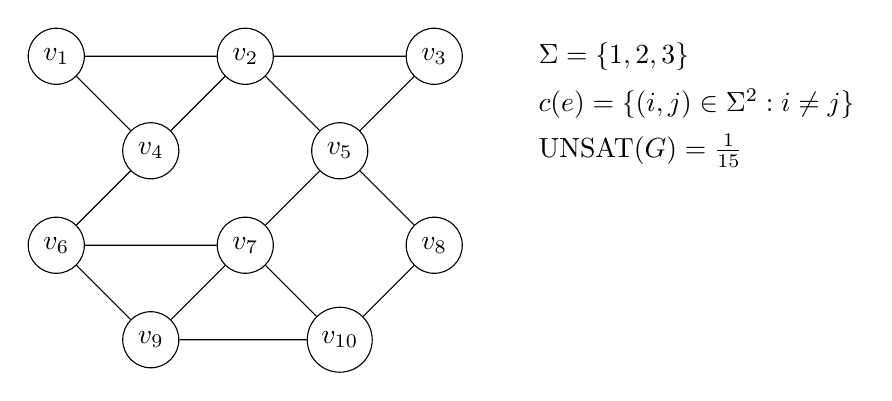
\begin{tikzpicture}[scale=1.2]
      % 頂点の定義
      \node[circle,draw,fill=white] (v1) at (0,3) {$v_1$};
      \node[circle,draw,fill=white] (v2) at (2,3) {$v_2$};
      \node[circle,draw,fill=white] (v3) at (4,3) {$v_3$};
      \node[circle,draw,fill=white] (v4) at (1,2) {$v_4$};
      \node[circle,draw,fill=white] (v5) at (3,2) {$v_5$};
      \node[circle,draw,fill=white] (v6) at (0,1) {$v_6$};
      \node[circle,draw,fill=white] (v7) at (2,1) {$v_7$};
      \node[circle,draw,fill=white] (v8) at (4,1) {$v_8$};
      \node[circle,draw,fill=white] (v9) at (1,0) {$v_9$};
      \node[circle,draw,fill=white] (v10) at (3,0) {$v_{10}$};
      
      % 辺の定義
      \draw (v1) -- (v2) -- (v3) -- (v5) -- (v2);
      \draw (v1) -- (v4) -- (v2);
      \draw (v4) -- (v6) -- (v7) -- (v5);
      \draw (v7) -- (v9) -- (v10) -- (v8) -- (v5);
      \draw (v6) -- (v9);
      \draw (v7) -- (v10);
      
      % 凡例
      \node[anchor=west] at (5,3) {$\Sigma = \{1,2,3\}$};
      \node[anchor=west] at (5,2.5) {$c(e) = \{(i,j) \in \Sigma^2 : i \neq j\}$};
      \node[anchor=west] at (5,2) {$\mathrm{UNSAT}(G) = \frac{1}{15}$};
    \end{tikzpicture}
    \caption{3彩色問題の制約グラフの例. 各頂点は3色のいずれかで彩色される必要があり, 隣接する頂点は異なる色でなければならない. この例では最適な彩色でも少なくとも1つの辺の制約を違反する必要があり, その割合は$\frac{1}{15}$となる.}
    \label{fig:3-coloring-constraint-graph}
  \end{figure}

\subsection{前処理補題}

PCP定理の証明の最初のステップは, 任意のCSPインスタンスを制約グラフに変換する前処理補題である. この変換は, 元のCSPの充足可能性と不満足値の基本的な性質を保持しつつ, 制約グラフの形式に変換する.

\begin{lemma}{前処理補題}{preprocessing-lemma}
  任意の$q$-CSPインスタンス$\varphi$に対して, 以下の性質を満たす制約グラフ$G$を多項式時間で構築できる:
  \begin{itemize}
  \item $\varphi$がYesインスタンスであることと, $\mathrm{UNSAT}(G) = 0$であることは同値である.
  \item $\varphi$がNoインスタンスであるとき, $\mathrm{UNSAT}(G) \ge \frac{1-\val(\varphi)}{q}$である.
  \item グラフ$G$の頂点数は$\abs{V} = O(n)$である.
  \item グラフ$G$の辺数は$\abs{E} = O(m)$である.
  \item アルファベット$\Sigma$は元のCSPと同じである.
  \end{itemize}
\end{lemma}

この補題の証明は, CSPインスタンスの制約を辺の制約に変換する単純な構築法に基づく. 具体的には, 各制約$c_i$に対して, その制約に含まれる変数間の辺を追加し, その辺に制約$c_i$を付随させる. この変換により, CSPの充足可能性と不満足値の基本的な性質が保持される.

前処理補題は, 任意のCSPインスタンスを制約グラフの形式に変換することで, 以降のギャップ増幅ステップのための準備を行う. この変換は多項式時間で実行可能であり, 元のCSPの重要な性質を保持するため, PCP定理の証明の基礎となる.

\section{エクスパンダーグラフ}
\subsection{エクスパンダーグラフの定義}

エクスパンダーグラフは, グラフの接続性を定量的に表現する重要な概念である. 特に, 任意の部分集合に対して, その境界のサイズが部分集合のサイズに応じて十分大きいという性質を持つ.

\begin{definition}{エクスパンダーグラフ}{expander-graph}
  $d$-正則グラフ$G=(V,E)$が\emph{$(n,d,\lambda)$-エクスパンダー}であるとは, 以下の条件を満たすことである:
  \begin{itemize}
  \item $\abs{V}=n$である.
  \item 任意の頂点の次数が$d$である.
  \item 任意の$S\subseteq V$に対して, $\abs{S}\le n/2$のとき
    \begin{align*}
      \abs{E(S,\overline{S})} \ge \lambda \cdot d \cdot \abs{S}
    \end{align*}
    が成り立つ. ここで, $E(S,\overline{S})$は$S$と$\overline{S}$を結ぶ辺の集合である.
  \end{itemize}
\end{definition}

エクスパンダーグラフの重要な性質として, ランダムウォークの収束が速いことが知られている. これは, エクスパンダーグラフのスペクトルギャップが大きいことと密接に関連している.

\subsection{エクスパンダー混交補題}

エクスパンダー混交補題は, エクスパンダーグラフにおけるランダムウォークの収束性を定量的に表現する重要な結果である.

\begin{lemma}{エクスパンダー混交補題}{expander-mixing-lemma}
  $(n,d,\lambda)$-エクスパンダー$G=(V,E)$を考える. 任意の$S,T\subseteq V$に対して
  \begin{align*}
    \abs{E(S,T)} - \frac{d}{n}\abs{S}\abs{T} \le \lambda\sqrt{\abs{S}\abs{T}}
  \end{align*}
  が成り立つ.
\end{lemma}

\begin{proof}
  隣接行列$A$の固有値を$\lambda_1\ge\lambda_2\ge\cdots\ge\lambda_n$とする. このとき, $\lambda_1=d$であり, $\lambda_2\le\lambda$であることが知られている.
  
  任意の$S,T\subseteq V$に対して, 特性ベクトル$\chi_S,\chi_T$を考える. このとき
  \begin{align*}
    \abs{E(S,T)} = \chi_S^\top A\chi_T
  \end{align*}
  が成り立つ. また, $\chi_S$と$\chi_T$を$A$の固有ベクトルで展開すると
  \begin{align*}
    \chi_S = \sum_{i=1}^n \alpha_i v_i, \quad \chi_T = \sum_{i=1}^n \beta_i v_i
  \end{align*}
  となる. ここで, $v_i$は$A$の固有ベクトルである.
  
  このとき
  \begin{align*}
    \abs{E(S,T)} - \frac{d}{n}\abs{S}\abs{T} &= \chi_S^\top A\chi_T - \frac{d}{n}\abs{S}\abs{T} \\
    &= \sum_{i=1}^n \lambda_i\alpha_i\beta_i - \frac{d}{n}\abs{S}\abs{T} \\
    &= \sum_{i=2}^n \lambda_i\alpha_i\beta_i \\
    &\le \lambda\sum_{i=2}^n \abs{\alpha_i\beta_i} \\
    &\le \lambda\sqrt{\sum_{i=2}^n \alpha_i^2}\sqrt{\sum_{i=2}^n \beta_i^2} \\
    &\le \lambda\sqrt{\abs{S}\abs{T}}
  \end{align*}
  が成り立つ.
\end{proof}

エクスパンダー混交補題は, エクスパンダーグラフにおける辺の分布が一様であることを示している. これは, PCP定理の証明において, 制約システムの不満足値を増幅する際に重要な役割を果たす.

\section{制約グラフのエクスパンダー化}

制約グラフのエクスパンダー化は, PCP定理の証明における重要なステップである. この変換により, 制約グラフの不満足値を増幅することが可能となる.

\begin{lemma}{制約グラフのエクスパンダー化}{constraint-graph-expander}
  制約グラフ$G=\langle(V,E),\Sigma,C\rangle$に対して, 以下の性質を満たす制約グラフ$G'=\langle(V',E'),\Sigma,C'\rangle$を多項式時間で構築できる:
  \begin{itemize}
  \item 基礎グラフ$(V',E')$は$(n',d',\lambda')$-エクスパンダーである. ここで, $n'=O(n)$, $d'=O(1)$, $\lambda'=O(1/\sqrt{d'})$である.
  \item $\mathrm{UNSAT}(G') \ge \Omega(\mathrm{UNSAT}(G))$である.
  \item アルファベット$\Sigma$は元のグラフと同じである.
  \end{itemize}
\end{lemma}

\begin{proof}
  制約グラフ$G$をエクスパンダーに変換する方法を説明する. 主なアイデアは, グラフの冪乗操作を用いて接続性を向上させることである.

  \emph{グラフの冪乗操作:}
  制約グラフ$G$の$t$乗$G^t$を以下のように定義する:
  \begin{itemize}
  \item 頂点集合は元のグラフと同じ$V$である.
  \item 辺$(u,v)$は, $G$上で$u$から$v$への長さ$t$のパスが存在する場合に存在する.
  \item 各辺$e'$の制約$c'(e')$は, 対応するパス上の制約の合成である. すなわち, パス$e_1,\dots,e_t$に対して
    \begin{align*}
      c'(e') = \{(a,b) \in \Sigma^2 : \exists a_1,\dots,a_{t-1} \in \Sigma, (a,a_1) \in c(e_1), (a_1,a_2) \in c(e_2), \dots, (a_{t-1},b) \in c(e_t)\}
    \end{align*}
    と定義する.
  \end{itemize}

  この冪乗操作により, グラフの接続性が向上し, エクスパンダー性が得られる. 具体的には, 以下の性質が成り立つ:

  \begin{lemma}{}{}
    制約グラフ$G$の$t$乗$G^t$は, 元のグラフ$G$の接続性を$t$倍に増幅する. すなわち, 任意の$S\subseteq V$に対して
    \begin{align*}
      \abs{E_{G^t}(S,\overline{S})} \ge t \cdot \abs{E_G(S,\overline{S})}
    \end{align*}
    が成り立つ.
  \end{lemma}

  \begin{proof}[Lemmaの証明]
    任意の$S\subseteq V$を考える. $G$上の$S$と$\overline{S}$を結ぶ辺の数を$k$とする.
    このとき, $G^t$上では, これらの辺を通る長さ$t$のパスが少なくとも$k$個存在する.
    各パスは$G^t$上の辺に対応するため, $E_{G^t}(S,\overline{S})$のサイズは少なくとも$k$である.
  \end{proof}

  次に, 不満足値の関係を証明する:

  \begin{lemma}{}{}
    $\mathrm{UNSAT}(G^t) \ge \Omega(t \cdot \mathrm{UNSAT}(G))$が成り立つ.
  \end{lemma}

  \begin{proof}[Lemmaの証明]
    任意の割り当て$\sigma: V \rightarrow \Sigma$を考える. $G$上の不満足な辺の割合を$\epsilon$とする.
    このとき, $G^t$上の任意の辺$e'$は, $t$個の$G$上の辺の制約の合成である.
    これらの制約のうち少なくとも$\epsilon t$個が不満足であるため,
    $\mathrm{UNSAT}_{\sigma}(G^t) \ge \Omega(\epsilon t)$が成り立つ.
  \end{proof}

  最後に, 適切な$t$を選択することで, 所望のエクスパンダー性が得られることを示す.
  $t=O(\log n)$とすると, グラフ$G^t$は$(n',d',\lambda')$-エクスパンダーとなる.
  ここで, $n'=n$, $d'=d^t=O(1)$, $\lambda'=O(1/\sqrt{d'})$である.
\end{proof}

この補題により, 任意の制約グラフをエクスパンダーに変換しつつ, 不満足値を保持することができる.
これは, PCP定理の証明におけるギャップ増幅ステップの基礎となる.